\chapter{Sezione d'urto}
Lo scattering è un tema fondamentale della fisica moderna utilizzato per rivelare la struttura della
materia, le proprietà delle particelle fondamentali e via discorrendo. \\
Con il termine scattering indichiamo tutti quei processi dove alcune particelle nello stato
iniziale interagiscono dando come risultato le stesse particelle oppure creandone altre
( esempio il collider è un processo di scattering ).
\section{Prima definizione di sezione d'urto}
Prendiamo un flusso di particelle " proiettile " che incide contro un bersaglio fisso fermo
il quale ha un determinato numero di nuclei per unità di volume : 
\begin{align*}
        \dot{N_{r}} &= \text{numero di reazioni per unità di tempo}\\
        \dot{N_{p}} &= \text{rate dei proiettili}\\
        n_{b} &= \text{numero nuclei per unità di volume}
\end{align*}
\begin{figure}[!h]
        \centering
        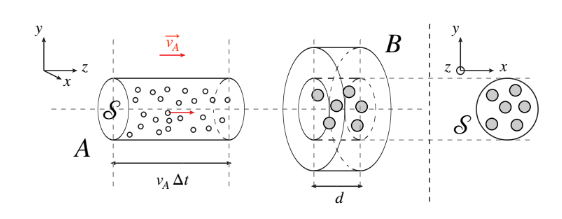
\includegraphics[scale=0.5]{ch4SezioneUrto/Scattering}
        \caption{Figura rubata dalle mitiche dispende del professor Kado}
\end{figure}
\newpage
Indichiamo il flusso di particelle che attraversazione la sezione trasversale S del bersaglio:
\begin{align*}
    \Phi = \dot{N_{p}}\frac{1}{S}
\end{align*}
Mentre il numero di particelle $N_{b}$ viste dai proiettili è :
\begin{align*}
    N_{b} = n_{b}Sd
\end{align*}
possiamo dire quindi con certezza che il rate di interazioni che avvengono è proporzionale 
a questi due termini : 
\begin{align*}
        \dot{N_{r}} &\propto \Phi N_{b} \\
                    &\propto \dot{N_{p}}n_{b}d
\end{align*}
ed è quì che entra in gioco la \textbf{sezione d'urto}, ossiamo come \textbf{coefficiente di  \\ proporzionalità}
\begin{align*}
    &\dot{N_{r}} = \sigma_{r}\dot{N_{p}}n_{b}d \\
    &\sigma_{r} = \frac{\dot{N_{r}}}{\dot{N_{r}}n_{b}d} \\
    &[\sigma_{r}] = \text{lunghezza}^{2} = \text{superficie}
\end{align*}
Indichiamo con \textbf{Luminosità istantanea} : 
\begin{align*}
    &L_{ist} = \dot{N_{p}}n_{b}d \\
    &[L_{ist}] = cm^{-2}s^{-1} 
\end{align*}
La luminosità è utile quando si lavora in processi di scattering fra due fasci di particelle
poichè si può scrivere in funzione del numero di particelle : 
\begin{align*}
    L = \frac{N_{a}N_{b}}{s}f_{rev} \tag*{$f_{rev}$ è la frequenza di rivoluzione}
\end{align*}
\subsection{Interpretazione geometrica}
La probabilità che una reazione avvenga è data da $\frac{\dot{N_{r}}}{\dot{N_{p}}}$, in un 
visione semplificata possiamo esprimere la probabilità come rapporto fra la superficie del 
proiettile e quella del bersaglio:
\begin{align*}
P = \frac{S_{r}}{S} = \frac{S_{eff}N_{b}}{S} \tag*{S = superficie flusso} \\ \tag*{$S_{eff}$ = superficie singolo bersaglio}
\end{align*}
si ottiene, ricordando la definizione di $N_{b}$ : 
\begin{align*}
        &\frac{\dot{N_{r}}}{\dot{N_{p}}} = S_{eff}n_{b}d \\
        &\sigma = S_{eff}
\end{align*}
tale interazione però non è del tutto esatta, infatti se prendiamo come bersaglio un protone 
e lo bombardiamo con diverse particelle si ottiene le sezioni d'urto sono differenti seppur
la $S_{eff}$ è sempre la stessa.
\newpage
\section{Una visione più sperimentale}
In un eseperimento quello che si fa è far interagire due fasci di particelle A e B, si pone 
un rivelatore in un certo punto dello spazio e si misurano il numero di interazioni per unità di tempo
che avvengono, da cosa dipende questo numero ? 
\begin{itemize}
        \item dinamica dell'interazione, ossia la sezione d'urto ;
        \item natura del bersaglio : tanto più alte sono le particelle bersaglio tanto 
                più alto è questo numero;
        \item flusso di particelle.
\end{itemize}
Il numero di interazioni, come abbiamo visto, si calcola:
\begin{align*}
    \dot{N_{r}} = \sigma_{r}\dot{N_{p}}n_{b}d
\end{align*}
\subsection{Come calcoliamo $n_{b}$}
La risposta è semplice : 
\begin{align*}
        n_{b} = \rho\frac{N_{A}}{A}
\end{align*}
dove $N_{A}$ è il numero di Avogradro e A è il numero di massa del materiale.
\subsection{Come calcoliamo $\dot{N_{p}}$}
Ovviamente non possiamo metterci a contare le particelle che passano per unità di tempo 
ma quello che si può fare è, conoscendo la carice delle particelle proiettile, ricavarci la 
corrente infatti : 
\begin{align*}
    i = \dv{q}{t} = q\dot{N_{p}}
\end{align*}
Facciamo un esempio : si ha un fascio di particelle $\alpha$ con carica i = 15 nA, calcoliamo 
$\dot{N_{p}}$. \\
\begin{align*}
        i = \dv{q_{\alpha}}{t} = q_{\alpha}\dot{N_{p}}
\end{align*}
ma, trattandosi di particelle $\alpha$, ossia nuclei di Elio, $q_{\alpha} = 2\abs{e}$ 
dove $\abs{e} = 1,6\times10^{-19}C$, ora dobbiamo trasformare i nA in $\frac{C}{s}$ : 
\begin{align*}
    1nA = 1\times10^{-9}A = 1\times10^{-9}\frac{C}{s}
\end{align*}
ed il gioco è fatto.
\newpage
